\begin{center}
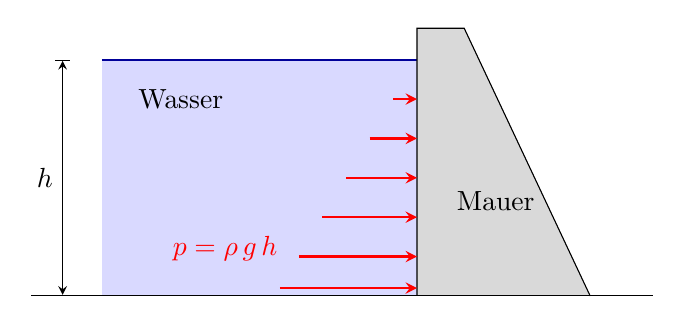
\begin{tikzpicture}[>=stealth]
 \fill[blue!15] (0,0) rectangle (4,3);
 \draw[blue!60!black, thick] (0,3) -- (4,3);
 \node at (1,2.5) {Wasser};
 \fill[gray!30] (4,0) -- (4,3.4) -- (4.6,3.4) -- (6.2,0) -- cycle;
 \draw (4,0) -- (4,3.4) -- (4.6,3.4) -- (6.2,0);
 \node at (5,1.2) {Mauer};
 \draw (-0.9,0) -- (7,0);
 \foreach \y in {2.5,2,1.5,1,0.5,0.1} \draw[->, red, thick] ({4-0.6*(3-\y)},\y) -- (4,\y);
 \node[red, anchor=east] at (2.35,0.6) {$p = \rho\,g\,h$};
 \draw[|<->|] (-0.5,3) -- (-0.5,0) node[midway, left] {$h$};
\end{tikzpicture}
\end{center}

Der Schweredruck $p = \rho\,g\,h$ nimmt linear mit der Wassertiefe $h$ zu. Auf jeden Quadratmeter der Mauer drückt das Wasser deshalb unten viel stärker als oben (rote Pfeile). Damit die Mauer diesen Kräften standhält, muss sie unten dicker sein; oben, wo der Druck klein ist, genügt eine dünne Mauer.

Die Form und die Grösse des Stausees spielen \result{\text{keine Rolle}}: Der Druck hängt nur von der Tiefe unter der Wasseroberfläche ab, nicht davon, wie viel Wasser hinter der Mauer liegt (hydrostatisches Paradoxon). Die Belastung der Mauer ist allein durch die Wasserhöhe an der Mauer und die Länge der Mauer bestimmt. Eine Mauer der Länge $b$ und der Wassertiefe $h$ wird mit der Kraft $F = \frac{1}{2}\rho\,g\,h^2\,b$ belastet (mittlerer Druck $\frac{1}{2}\rho\,g\,h$ mal Fläche $h\,b$), egal ob dahinter ein schmaler Kanal oder ein grosser See liegt.
